\documentclass[11pt]{article}
\usepackage[utf8]{inputenc}

\title{API Javascript for ArcGIS}
\author{Clément Delgrange}
\date{Avril 2018}

% Modules generaux
\usepackage[T1]{fontenc}
\usepackage[francais]{babel} % prise en charge du francais
\usepackage[table]{xcolor} % tableaux
\usepackage{graphicx} % images
\usepackage{float}
\usepackage[font=small]{caption}

% Marges
\usepackage[left=2cm,right=2cm,top=2cm,bottom=2cm]{geometry}

% Personnalisation des titres
\usepackage{titlesec}
\titlespacing{\section}{0em}{4em}{1em}
\titlespacing{\subsection}{0em}{2em}{0em}
\titlespacing{\subsubsection}{0em}{0.5em}{0em}

% Mise en page
\setlength{\parskip}{1.2em}
\renewcommand{\floatpagefraction}{1}

% Couleurs personnalisées
\usepackage{color}
\definecolor{lightgray}{gray}{0.98}
\definecolor{gray}{rgb}{0.6, 0.6, 0.65}
\definecolor{green}{rgb}{0.133, 0.545, 0.133}
\definecolor{blue}{rgb}{0, 0, 1}
\definecolor{red}{rgb}{0.6, 0.1, 0.1}

% Liens hypertextes
\usepackage{hyperref}
\hypersetup{
	colorlinks=true,
	breaklinks=true,
	urlcolor=blue,
	linkcolor=blue,
	pdfborder=000,
	pdftex=true
}

% Mise en forme des codes javascript
\usepackage{listingsutf8}
\lstdefinelanguage{JavaScript}{
  keywords={typeof, new, true, false, catch, function, return, null, catch, switch, var, if, in, while, do, else, case, break},
  keywordstyle=\color{blue}\bfseries,
  ndkeywords={class, export, boolean, throw, implements, import, this},
  ndkeywordstyle=\color{darkgray}\bfseries,
  identifierstyle=\color{black},
  sensitive=false,
  comment=[l]{//},
  morecomment=[s]{/*}{*/},
  commentstyle=\color{purple}\ttfamily,
  stringstyle=\color{red}\ttfamily,
  morestring=[b]',
  morestring=[b]"
}
\lstset{
	language=JavaScript,
	keywordstyle=\bfseries\ttfamily\color{blue},
	identifierstyle=\ttfamily,
	commentstyle=\color{gray},
	stringstyle=\ttfamily\color{green},
	showstringspaces=false,
	basicstyle=\footnotesize\ttfamily,
	tabsize=2,
	breaklines=true,
	extendedchars=true,
	xleftmargin=1cm,
	xrightmargin=1cm,
	backgroundcolor=\color{lightgray},
	literate=%
		{é}{{\'{e}}}1
		{è}{{\`{e}}}1
		{ê}{{\^{e}}}1
		{ë}{{\¨{e}}}1
		{û}{{\^{u}}}1
		{ù}{{\`{u}}}1
		{â}{{\^{a}}}1
		{à}{{\`{a}}}1
		{î}{{\^{i}}}1
		{ô}{{\^{o}}}1
		{ç}{{\c{c}}}1
}

% Commandes personnalisées
\newcommand{\bslash}{\texttt{\symbol{92}}}
\newcommand{\action}{$\Rightarrow$ }
\newcommand{\reponse}{
	\begin{tabbing}
	\hspace{2cm}\=\kill
	Réponse \> ............................................................................................ \\
 	\> ............................................................................................
	\end{tabbing}
}

\newenvironment{note}{%
	\begin{tabular}[t t]{c c}
		
\includegraphics{img/tips.png}
		 &
		\begin{minipage}[c]{0.9\linewidth}
			\begin{sffamily}
}{%
			\end{sffamily}
		\end{minipage}
	\end{tabular}
}

\newenvironment{objectifs}{
  \hrule
	\begin{minipage}{0.9\textwidth}
		\vspace{1em}
		\begin{tabular}[t t]{c c}
			
\includegraphics[width=0.1\linewidth]{img/goals.jpg} &
			\begin{minipage}[c]{0.8\linewidth}
				\hspace{2em}\textbf{\large{Objectifs :}} \\
}{
			\end{minipage}
		\end{tabular}
		\vspace{1em}
	\end{minipage}
	\hrule
}

\newcommand{\code}[1]{\lstinline{#1}}

\newenvironment{python}{%
	\begin{lstlisting}
}{%
	\end{lstlisting}
}

% Entetes et pieds de page
\usepackage{fancyhdr}
\pagestyle{fancy}
\fancyhf{}
\renewcommand{\headrulewidth}{0pt}
\makeatletter
\fancyfoot[L]{\@author}
\fancyfoot[C]{-\thepage-}
\fancyfoot[R]{\@title}
\makeatother
\renewcommand{\footrulewidth}{0.5pt}


%%%%%%%%%%%%
%%% Document
%%%%%%%%%%%%
\begin{document}
\parindent=0cm


\begin{titlepage}
\makeatletter
	\begin{sffamily}
		\begin{flushleft}
			% 
\includegraphics{img/logos/ign-logo-ensg.jpg}\\[1.5cm]
		\end{flushleft}
		\begin{flushright}
			% pour mettre une image en haut à droite
		\end{flushright}

		\vspace{4cm}

		\begin{center}
			\hrule
				\vspace{1em}
				{\small \textit{Programmation SIG}}\\
				\vspace{0.5cm}
				{\huge\bfseries \@title}
				\vspace{1cm}
			\hrule

			\vspace{4cm}
			%\includegraphics[width=400px]{images/logo_python.png}
			\begin{objectifs}
			\begin{itemize}
				\item appendre les bases de l'API Javascript for ArcGIS
				\item réaliser des applications web SIG à l'aide de cette API
			\end{itemize}
			\end{objectifs}

			\vspace{3cm}

			\large \textit{\@author}\\
			\small \textit{\@date}
		\end{center}
	\end{sffamily}
\makeatother
\end{titlepage}



\section*{Préalables}
Les développements que vous réaliserez doivent être déposés sur un serveur web. 
Vous pouvez travailler en local en installant un serveur web sur votre ordinateur (installer WAMP ou EasyPHP sous windows).

Ce TD ne constitue qu'une introduction à l'API Javascript for ArcGIS, qui vous permettra de réaliser une web SIG relativement simple.
Pour aller plus loin dans la découverte de cette API, nous vous recommandons vivement de consulter la documentation en ligne, très claire et bien fournie en exemples : \url{https://developers.arcgis.com/javascript/}.

\subsection*{Ce que vous devez savoir en Javascript}
Une connaissance approfondie du langage JavaScript n'est pas nécessaire pour pouvoir suivre le TD.
Nous revenons dans cette introduction sur quelques spécificités du langage qui suffirons pour comprendre la suite du TD.

Le JavaScript est un langage interprété à typage dynamique faible. 
Il supporte de nombreux paradigmes de programmation : orienté objets, impératif, etc. 
Enfin, il n'a aucun rapport avec Java!

En règle général, le code JavaScript est utilisé dans le contexte des applications web où il est exécuté dans les navigateurs.

Pour insérer du code JavaScript dans une page web, nous disposons de deux méthodes :
\begin{itemize}
	\item l'écrire dans une balise \code{<script>} n'importe où dans la page HTML;
	\item l'écrire dans un fichier séparé qui sera lié à la page HTML grâce à une balise \code{<script>} avec un attribut \code{src}.
\end{itemize}

Généralement nous utiliserons la seconde méthode et nous placerons la balise à la fin du \code{<body>}.

Fichier HTML :
\begin{lstlisting}
<!DOCTYPE html>
<html>
<head>
    <title>Hello World!</title>
</head>
<body>
	<script type="text/javascript" src="helloworld.js"></script>
</body>
</html>
\end{lstlisting}

Fichier \code{helloworld.js} (qui ici ouvre une boîte de dialogue avec un message \textit{Hello world!}) :
\begin{lstlisting}
alert('Hello world!');
\end{lstlisting}

En JavaScript les instructions sont séparées par des points virgules. 
Pour le nommage des variables, le langage est sensible à la casse (\code{mavariable} est différent de \code{MaVariable}).

Il est possible d'insérer des commentaires de deux manières :
\begin{lstlisting}
//commentaire sur une ligne

/* Commentaires
sur plusieurs
lignes */
\end{lstlisting}

Pour afficher un message dans la console du navigateur (généralement la console s'affiche en activant les outils de développement de votre navigateur), nous écrirons :
\begin{lstlisting}
console.log(msg);
\end{lstlisting}

Déclaration et instanciation d'une variable sont deux opérations distinctes en JavaScript:
\begin{lstlisting}
var maVariable;  // déclaration
mavariable = 5;  // instanciation
\end{lstlisting}

Mais il est tout à fait possible des grouper ces deux opérations dans la même instruction :
\begin{lstlisting}
var maVariable = 5;
\end{lstlisting}

La syntaxe pour les boucles \textit{for} est :
\begin{lstlisting}
for(var i = 0; i < 5; i++) {
  alert('Itération n' + i);
}
\end{lstlisting}

Les objets JavaScript sont écrit à l'aide d'accolades.
Les propriétés sont décrites sous forme de \code{nom: valeur} :
\begin{lstlisting}
var objet = {
	param1: val1,
	param2: val2,
	...
});
\end{lstlisting}

Le concept de classes à également été introduit en JavaScript.
Pour définir une instance de classe, nous écrirons :
\begin{lstlisting}
var objet = new Classe({
	param1: val1,
	param2: val2,
	...
});
\end{lstlisting}

Les attributs d'un objet sont accessibles de la manière suivante :
\begin{lstlisting}
var objet = new Classe();
objet.param1 = val1;
objet.param2 = val2;
...
\end{lstlisting}

\newpage



\section{Premiers pas: afficher un fond de plan}
Pour commencer, nous allons afficher un fond de carte dans une application web.

\action Créez un fichier HTML basique contenant pour l'instant uniquement les lignes suivantes\footnote{La première balise meta indique que la suite de l'HTML sera encodée en UTF-8, tandis que la seconde permet de contrôler la mise en page sur les navigateurs mobiles.} :
\begin{lstlisting}
<!DOCTYPE html>
<html>
	<head>
		<meta charset="utf-8">
		<meta name="viewport" content="initial-scale=1, maximum-scale=1">
		<title>First Web SIG application</title>
	</head>
	<body>
	</body>
</html>
\end{lstlisting}

Pour utiliser l'API Javascript for ArcGIS, nous avons plusieurs possibilités :
\begin{itemize}
	\item la télécharger\footnote{\url{https://developers.arcgis.com/downloads/apis-and-sdks?product=javascript}} et la référencer en local dans la page HTML, ce qui est utile si vous souhaitez faire des tests alors que vous n'avez pas accès à internet;
	\item référencer l'API dans la page HTML en pointant vers le CDN (content delivery network), ce qui assure de travailler avec une version à jour de l'API;
	\item utiliser Bower, un gestionnaire de paquets pour le web, pour installer une version spécifique de l'API en local, ce qui est utile dans certaines configurations.
\end{itemize}

Nous utiliserons dans ce TD la deuxième solution.

\action Ajoutez les deux balises suivantes dans l'entête de l'HTML pour référencer l'API Javascript d'ArcGIS :
\begin{lstlisting}
<script src="https://js.arcgis.com/4.6/"></script>
<link rel="stylesheet" href="https://js.arcgis.com/4.6/esri/css/main.css">
\end{lstlisting}

\begin{note}
Nous utilisons ici la feuille de style par défaut d'Esri, mais il est possible d'en utiliser d'autres\footnote{\url{https://developers.arcgis.com/javascript/latest/guide/styling/index.html}}, voir de la personnaliser.
\end{note}

Il nous reste à ajouter le code permettant de charger les différents éléments de l'API.

\action Ajoutez une balise \code{<script type="text/javascript" src="script.js"></script>} juste avant la fermeture du \code{body} de votre page HTML, et créez le fichier JavaScript \code{script.js} dans le même répertoire que le HTML.

L'API JavaScript d'ArcGIS est basée sur la bibliothèque \textbf{Dojo Toolkit}, dont le principe de fonctionnement sera donc ici repris. 
Cela nous impactera en particulier pour un point : le mécanisme permettant d'importer des modules ou classes de l'API.
La syntaxe sera :
\begin{lstlisting}
require(["module1", "module2", ..., "dojo/domReady!"], function(Classe1, Classe2, ...) {
	/* écrire ici le code JavaScript pour afficher la carte */
});
\end{lstlisting}

\begin{note}
L'utilisation de \code{dojo/domReady} est équivalente à celle d'un attribut onLoad en HTML : le code ne s'exécute que lorsque le \textit{document object model} (DOM) est complètement chargé.
\end{note}

Pour créer une carte avec l'API, nous utiliserons la classe \code{Map} du module \code{esri/Map}. 
C'est elle qui permet de gérer les différentes couches affichées ou encore le fond de plan. 
Pour rendre visible la carte, elle doit être référencée dans un objet faisant le lien entre la carte et la balise HTML où l'afficher. 
Cet objet c'est le \code{MapView} du module \code{esri/views/Mapview}.

\action Ajoutez la fonction \code{require()} avec le bons paramètres à votre JavaScript.

La déclaration des objets \code{Map} et \code{MapView} s'effectue de la manière suivante :
\begin{lstlisting}
var myMap = new Map({
    basemap: "satellite"  // utilisation d'une image satellite comme fond de plan
});

var myView = new MapView({
	container: "viewDiv",  // affichage de la carte dans la balise viewDiv du html
	map: myMap
});
\end{lstlisting}

\action Recopiez ce code dans votre fonction \code{require()}.

Ces instructions spécifient entre autre que le contenu de la carte doit s'afficher dans une balise d'identifiant \code{viewDiv}.

\action Ajoutez cette balise dans le \code{body} de votre page HTML.

La carte contenue dans cette balise ne sera enfin visible que si vous lui imposez une taille minimale.

\action En référencant un fichier de style ou en ajoutant une balise \code{<style>}, précisez que la carte doit s'étendre sur toute l'étendue de la page (propriétés \code{height} et \code{width} à 100\%).

Vous pouvez enfin aller dans un navigateur pour tester votre application !

\begin{note}
Dans ce premier exemple, nous avons utilisé des options par défaut pour les objets \code{Map} et \code{MapView}, mais l'API permet de jouer sur de nombreux paramètres.

Pour la carte, nous pouvons par exemple changer le fond de plan : carte, image satellite, vue hybride, carte topo, OpenStreetMap, carte en niveau de gris, etc.

Pour la vue, il est possible de modifier le centre, le niveau de zoom, l'orientation, etc.

Consultez la documentation\footnote{\url{https://developers.arcgis.com/javascript/latest/api-reference/esri-views-MapView.html} et \url{https://developers.arcgis.com/javascript/latest/api-reference/esri-Map.html}} pour la liste complète des propriétés sur lesquelles il est possible de jouer.
\end{note}



\section{Passer à une vue 3D}
Les derniers versions de l'API Javascript for ArcGIS ont grandement simplifié la réalisation de scènes 3D. En effet, pour indiquer que l'on souhaite obtenir une vue 3D, il suffit d'utiliser une objet de type \code{SceneView} à la place de \code{MapView}. Et il n'y a rien de plus à faire !

\action En repartant de l'exemple précédent, réalisez une application web SIG affichant des images satellites sur un globe 3D.

\begin{note}
Ici encore, des options de l'objet \code{SceneView}\footnote{\url{https://developers.arcgis.com/javascript/latest/api-reference/esri-views-SceneView.html}} peuvent être spécifiées dans le code : centre, niveau de zoom, modèle d'élévation, etc.
\end{note}

Excepté ce petit changement, l'utilisation de l'API est identique que l'on désire travailler en 2D ou en 3D. Pour la suite de ce TD, nous resterons en vue 3D.



\section{Ajout d'une couche d'entités}
Pour l'instant, notre application web SIG est assez basique. Pour la rendre plus utile, nous allons commencer par y ajouter une couche d'entités (objet \code{FeatureLayer} du module \code{esri/layers/FeatureLayer}).

Pour ajouter une couche, l'API propose globalement deux approches :
\begin{itemize}
	\item intégrer la ressource en utilisant l'adresse de son protocole REST;
	\item dans le cas d'une ressource publiée sur ArcGIS Online (ou Portal for ArcGIS), utiliser son identifiant sur la plateforme.
\end{itemize}

Nous utiliserons ici la deuxième solution. La création de la \code{FeatureLayer} s'effectuera donc en passant un objet de type \code{PortalItem} au constructeur de \code{FeatureLayer} :
\begin{lstlisting}
var featureLayer = new FeatureLayer({
	portalItem: {
		id: "<arcgis_online_feature_layer_id>"
	}
});
\end{lstlisting}

Puis une fois la couche définie, nous l'ajoutons à la carte par \code{myMap.add(featureLayer);}.

Nous voulons ajouter le bâtiment publié dans une carte ArcGIS Online lors du TD précédent dans notre application web SIG. Il nous faut pour cela générer préalablement la couche d'entités correspondante dans ArcGIS Online.

\action Sur ArcGIS Online, ouvrez la carte web réalisée lors du TD précédent (contenu \textit{BatiENSG} de type \textit{Web Map}).

\action Cliquez sur les \code{...} après la couche \textit{Bâtiment ENSG} et sélectionnez \textbf{Enregistrer la couche}.
\begin{figure}[H]
	\center 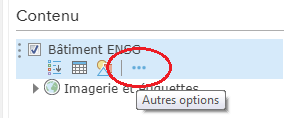
\includegraphics[width=0.3\textwidth]{img/td2/ago_enregistrer_couche.png} \\
\end{figure}

\action Revenez sur la page des contenus.

\action Ouvrez la ressource de type \textit{Feature Layer}.

L'identifiant ArcGIS Online se retrouve dans l'URL :
\begin{figure}[H]
	\center 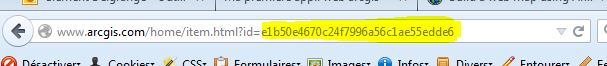
\includegraphics[width=0.8\textwidth]{img/td2/js_ago_mapid.jpg} \\
\end{figure}

\action En vous servant de la syntaxe donnée plus haut et de l'identifiant de la couche, ajoutez-la à votre application web SIG.

\begin{note}
Depuis le début de ce TD, nous créons une carte en définissant un fond de plan. Il n'est en fait pas obligatoire d'en utiliser un. Si aucun argument n'est passé au constructeur, les entités s'affichent sur un fond blanc :
\begin{figure}[H]
	\center 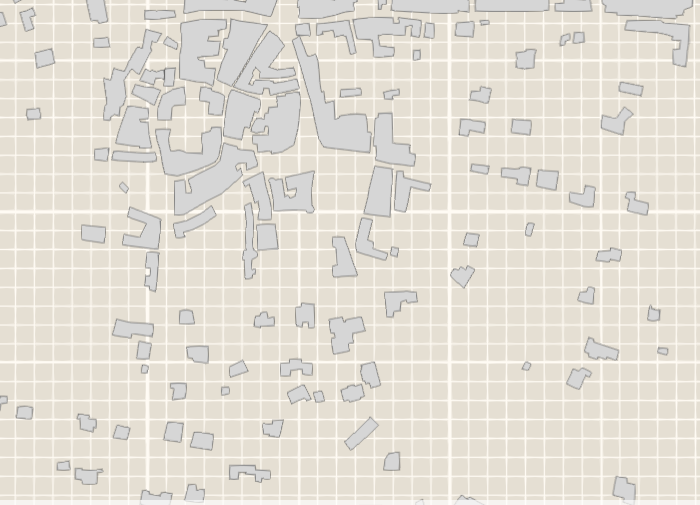
\includegraphics[width=0.4\textwidth]{img/td2/js_sans_fond_plan.png} \\
\end{figure}
\end{note}



\section{Déclencher une action après le chargement d'un objet}

\begin{lstlisting}
myView.then(function(){
	// Toutes les ressources de la vue myView ont été chargée

}, function(error){
	// Il y a eu un problème au chargement

});
\end{lstlisting}

Exemple : activer l'élévation d'une scène 3D

\begin{lstlisting}
map.ground.layers.forEach(function(layer) {
	layer.visible = true;
});
\end{lstlisting}

Pour plus d'intérêt (Champs-sur-Marne c'est un peu plat), vous pouvez utiliser la couche d'entités d'identifiant "0aca29c0e8d7447282ba205f6e0942e3" sur ArcGIS Online.


\section{Bâtiments en 3D}
Nous allons tenter de représenter les bâtiments en volume. Pour commencer, nous allons utiliser la même hauteur pour tous les bâtiments puis nous essayerons de tenir compte de leur hauteur réelle.

Le principe est le suivant :
\begin{itemize}
	\item définir un \code{ExtrudeSymbol3DLayer}\footnote{\url{https://developers.arcgis.com/javascript/latest/api-reference/esri-symbols-ExtrudeSymbol3DLayer.html}} en lui affectant une couleur et une taille raisonnable (10m);
	\item définir un \code{PolygonSymbol3D}\footnote{\url{https://developers.arcgis.com/javascript/latest/api-reference/esri-symbols-PolygonSymbol3D.html}} en utilisant comme couche de symboles l'\code{ExtrudeSymbol3DLayer} définie précédemment;
	\item appliquer à la couche des bâtiments un rendu de type \code{SimpleRenderer}\footnote{\url{https://developers.arcgis.com/javascript/latest/api-reference/esri-renderers-SimpleRenderer.html}}) avec comme symbole celui défini juste avant.
\end{itemize}

\begin{note}
Le principe est le même pour appliquer n'importe qu'elle symbologie à une couche : définir un symbol puis appliquer un rendu.
\end{note}

\action En vous aidant des différentes pages de la documentation, appliquez un rendu 3D aux bâtiments.

Pour faire varier la taille en fonction de la hauteur, nous allons jouer avec la propriété \code{visualVariables} de l'objet \code{SimpleRenderer}.

\action Regardez dans la documentation comment fonctionne cette propriété et modifiez votre code en conséquence.



\section{Ajout de widgets}
Les widgets sont des composants "clé-en-main" de l'API qui peuvent être utilisés dans une applications. Leurs champs d'actions sont assez variés : légende, popup, miniature, outils de mesure, de recherche ou de navigation, etc.

Nous ajouterons une légende à notre application. L'utilisation des autres widgets est similaire.

\action Définissez une légende à l'aide du code suivant :
\begin{lstlisting}
// on crée un nouveau widget (ici une légende)
var legend = new Legend({
  view: myView, // on indique à quelle vue s'applique le widget
  layerInfos: [{
    layer: featureLayer,
    title: "Bâtiment"
  }] // propriétés spécifiques au widget (ici : les couches et leurs noms)
});
\end{lstlisting}

\action Puis ajoutez la légende à la vue avec \code{myView.ui.add(legend, "bottom-right")}.


\end{document}
